
\documentclass[calculator,steamtables,refrigeranttables,psychrometricchart,datasheet,resit,solution]{exam}
%\documentclass[calculator,steamtables,refrigeranttables,psychrometricchart,datasheet]{exam}

% The full list of class options are
% calculator : Allows approved calculator use.
% datasheet : Adds a note that data sheet are attached to the exam.
% handbook : Allows the use of the engineering handbook.
% resit : Adds the resit markings to the paper.
% sample : Adds conspicuous SAMPLE markings to the paper
% solutions : Uses the contents of \solution commands (and \solmarks) to generate a solution file

\usepackage{pdfpages}
\usepackage{lscape,comment}

\coursecode{EG3521}%%
\coursetitle{Engineering Thermodynamics}%
%\coursecode{EG3539}% 
%\coursetitle{Thermodynamics}%

\examtime{00.00--00.00}%
\examdate{00}{05}{2015}%
\examformat{Candidates must attempt \textit{all} questions.}

\newcommand{\frc}{\displaystyle\frac}
\newcommand{\br}[1]{\!\left( #1 \right)}
\newcommand{\abs}[1]{\left| #1 \right|}
\newcommand{\fracd}[2]{\frac{\mathrm{d} #1}{\mathrm{d} #2}}
\newcommand{\fracp}[2]{\frac{\partial #1}{\partial #2}}
\renewcommand{\d}[1]{\mathrm{d} #1 }
\newcommand{\Ma}{\mathrm{M\!a}}



\begin{document}

\begin{question}
ioi
\end{question}



\paperend

%\begin{comment}
%\begin{landscape}
%\begin{center}
%\includegraphics[width=1.5\textwidth]{PsychrometricChart}
%\end{center}
%{
%  \includepdf[pages=-,fitpaper]{./Pics/PsychrometricChart}
%  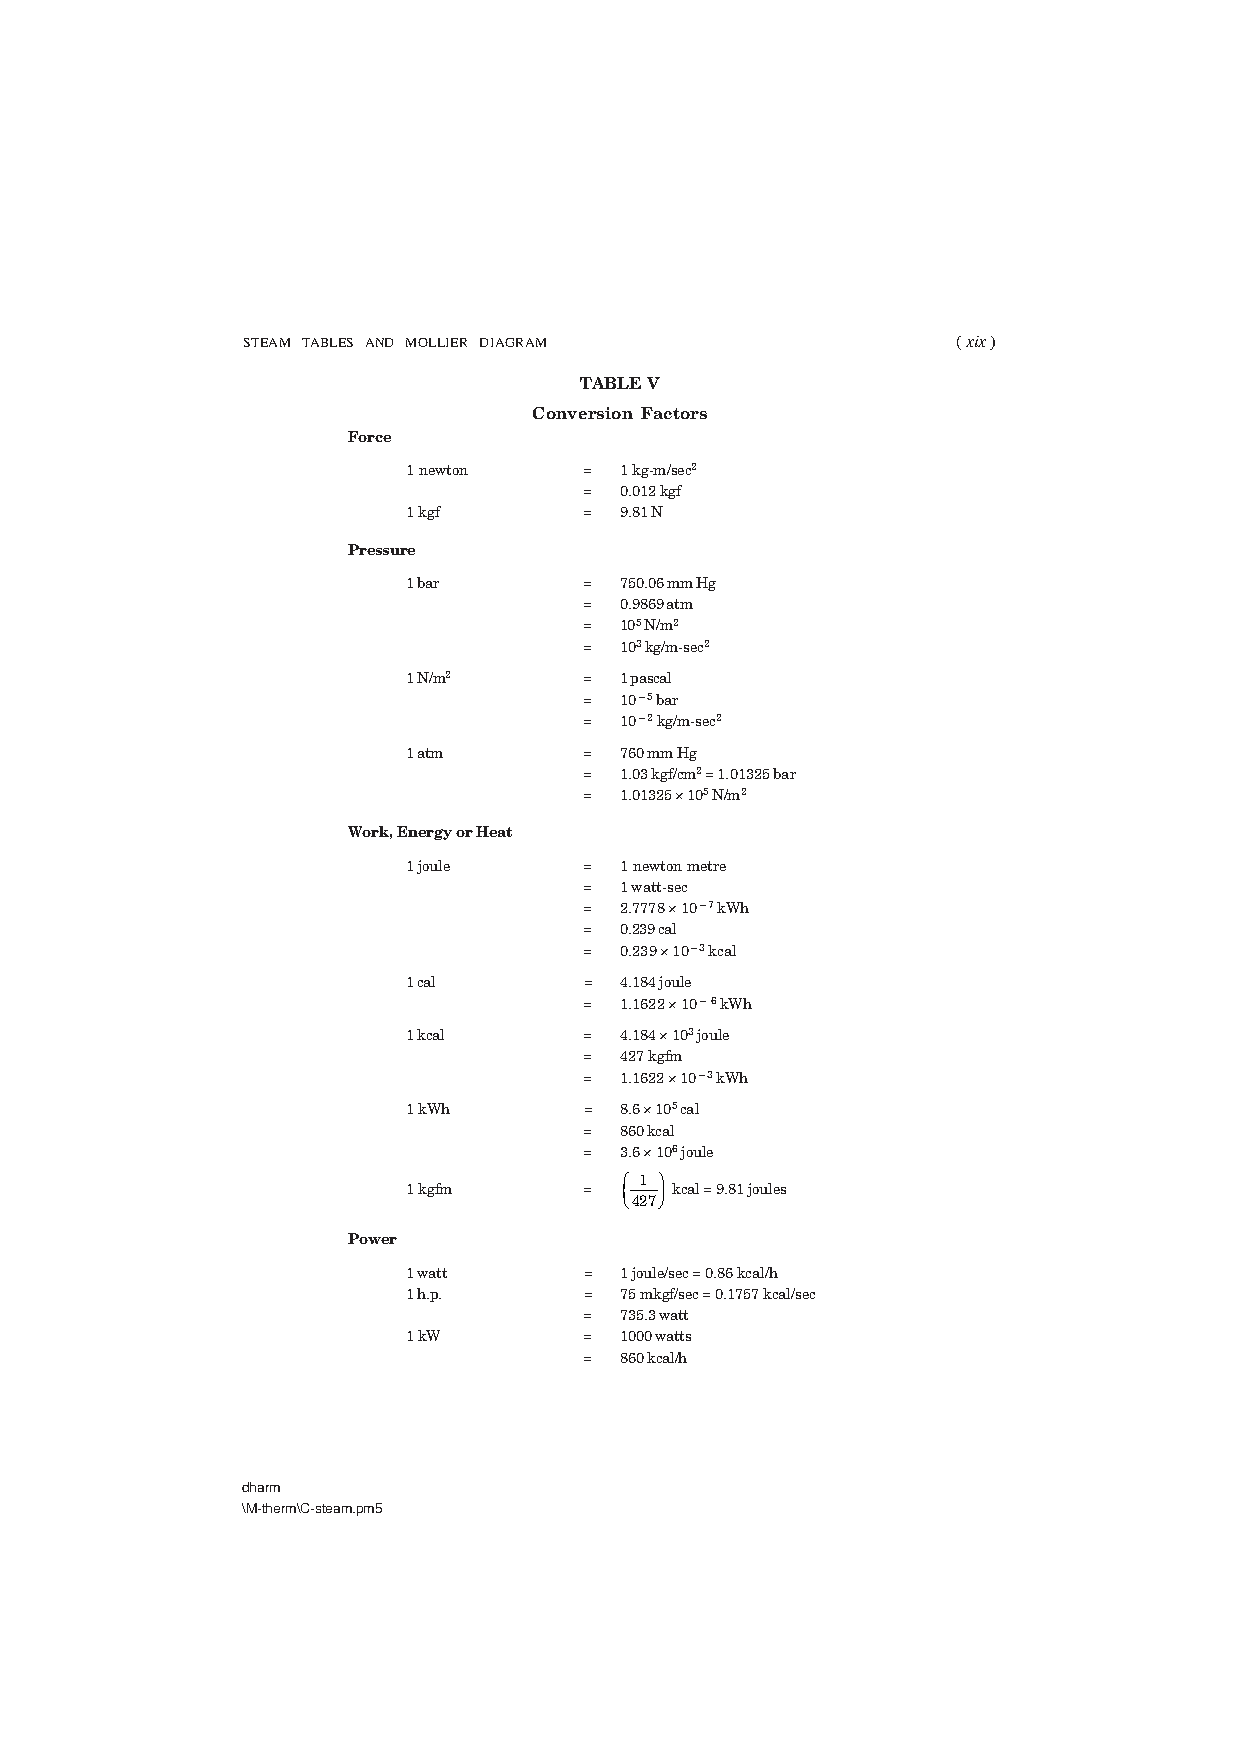
\includepdf[pages=-,fitpaper]{./Pics/UnitsConversion}
%  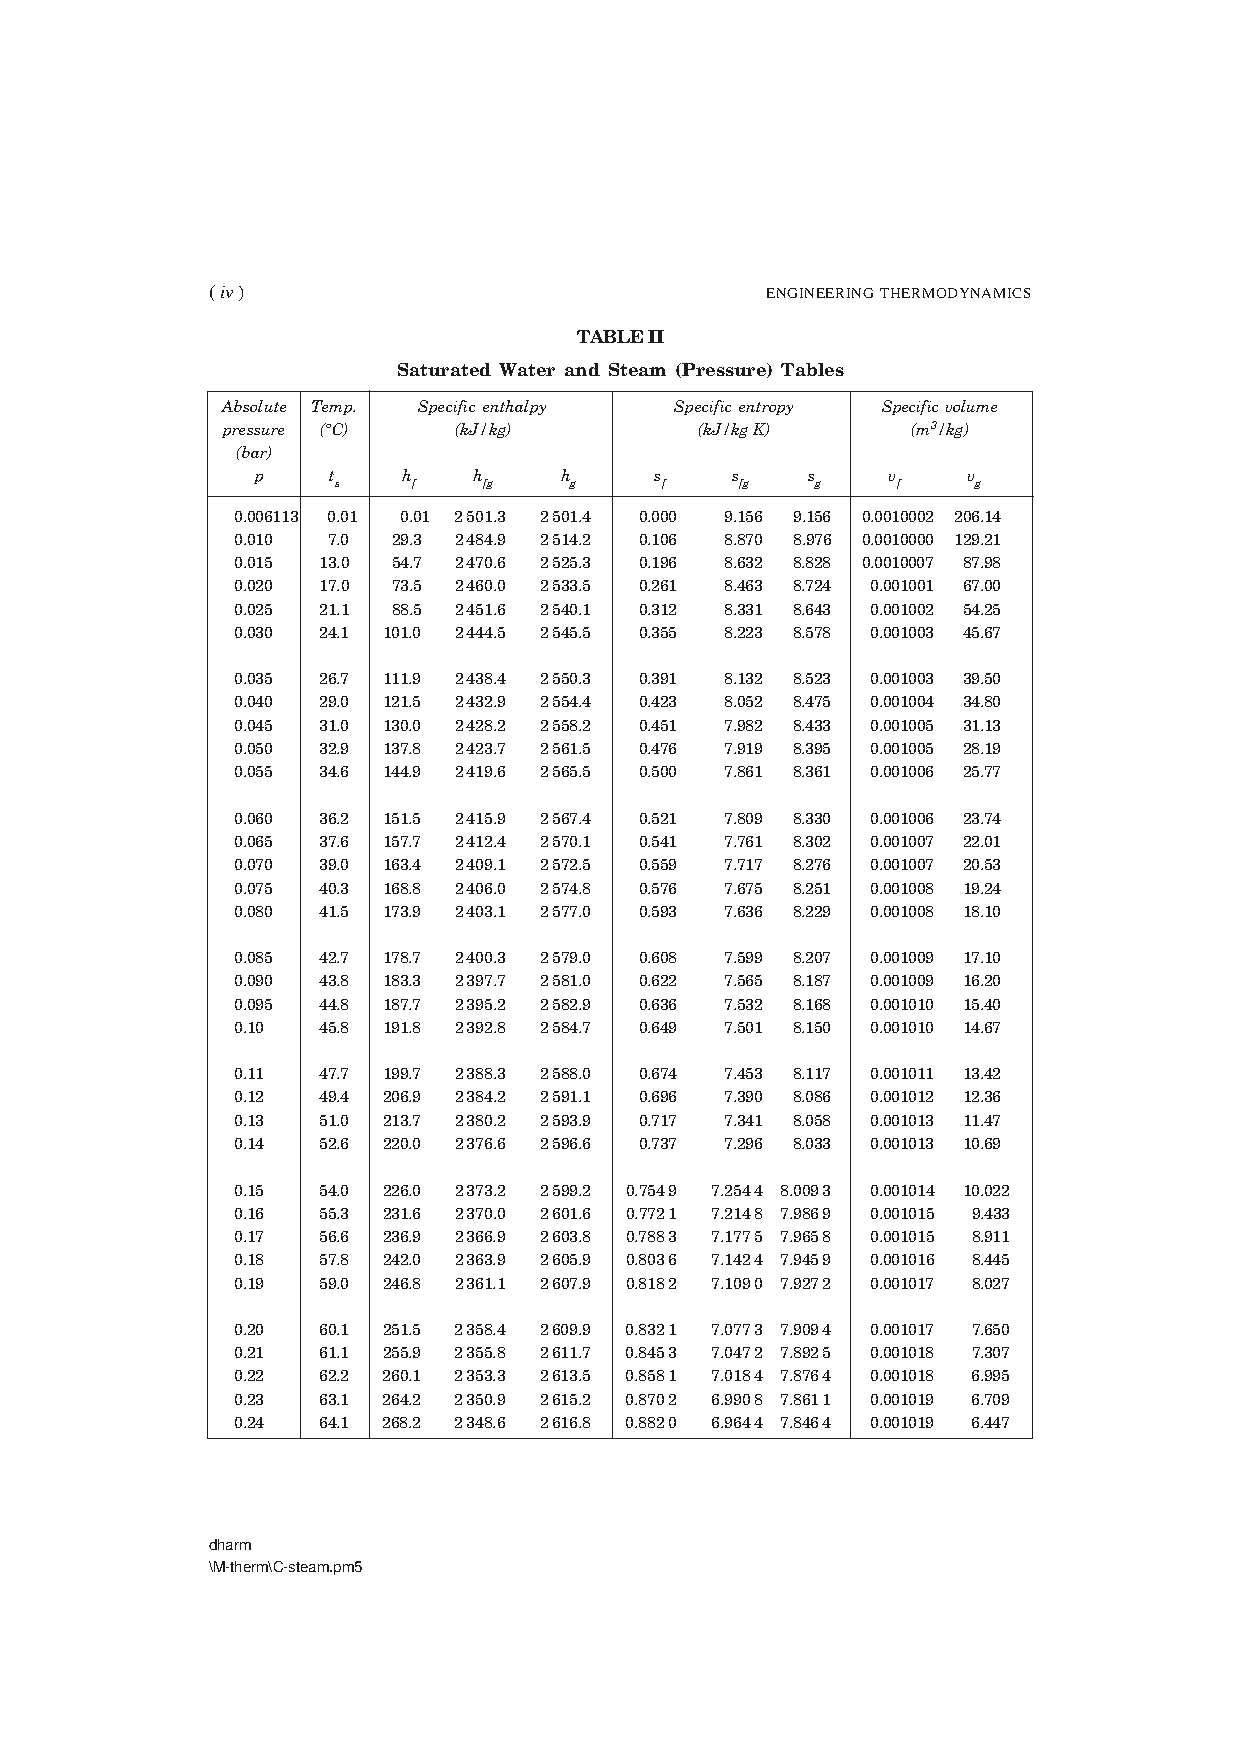
\includepdf[pages=-,fitpaper]{./Pics/SteamTable_2}
%  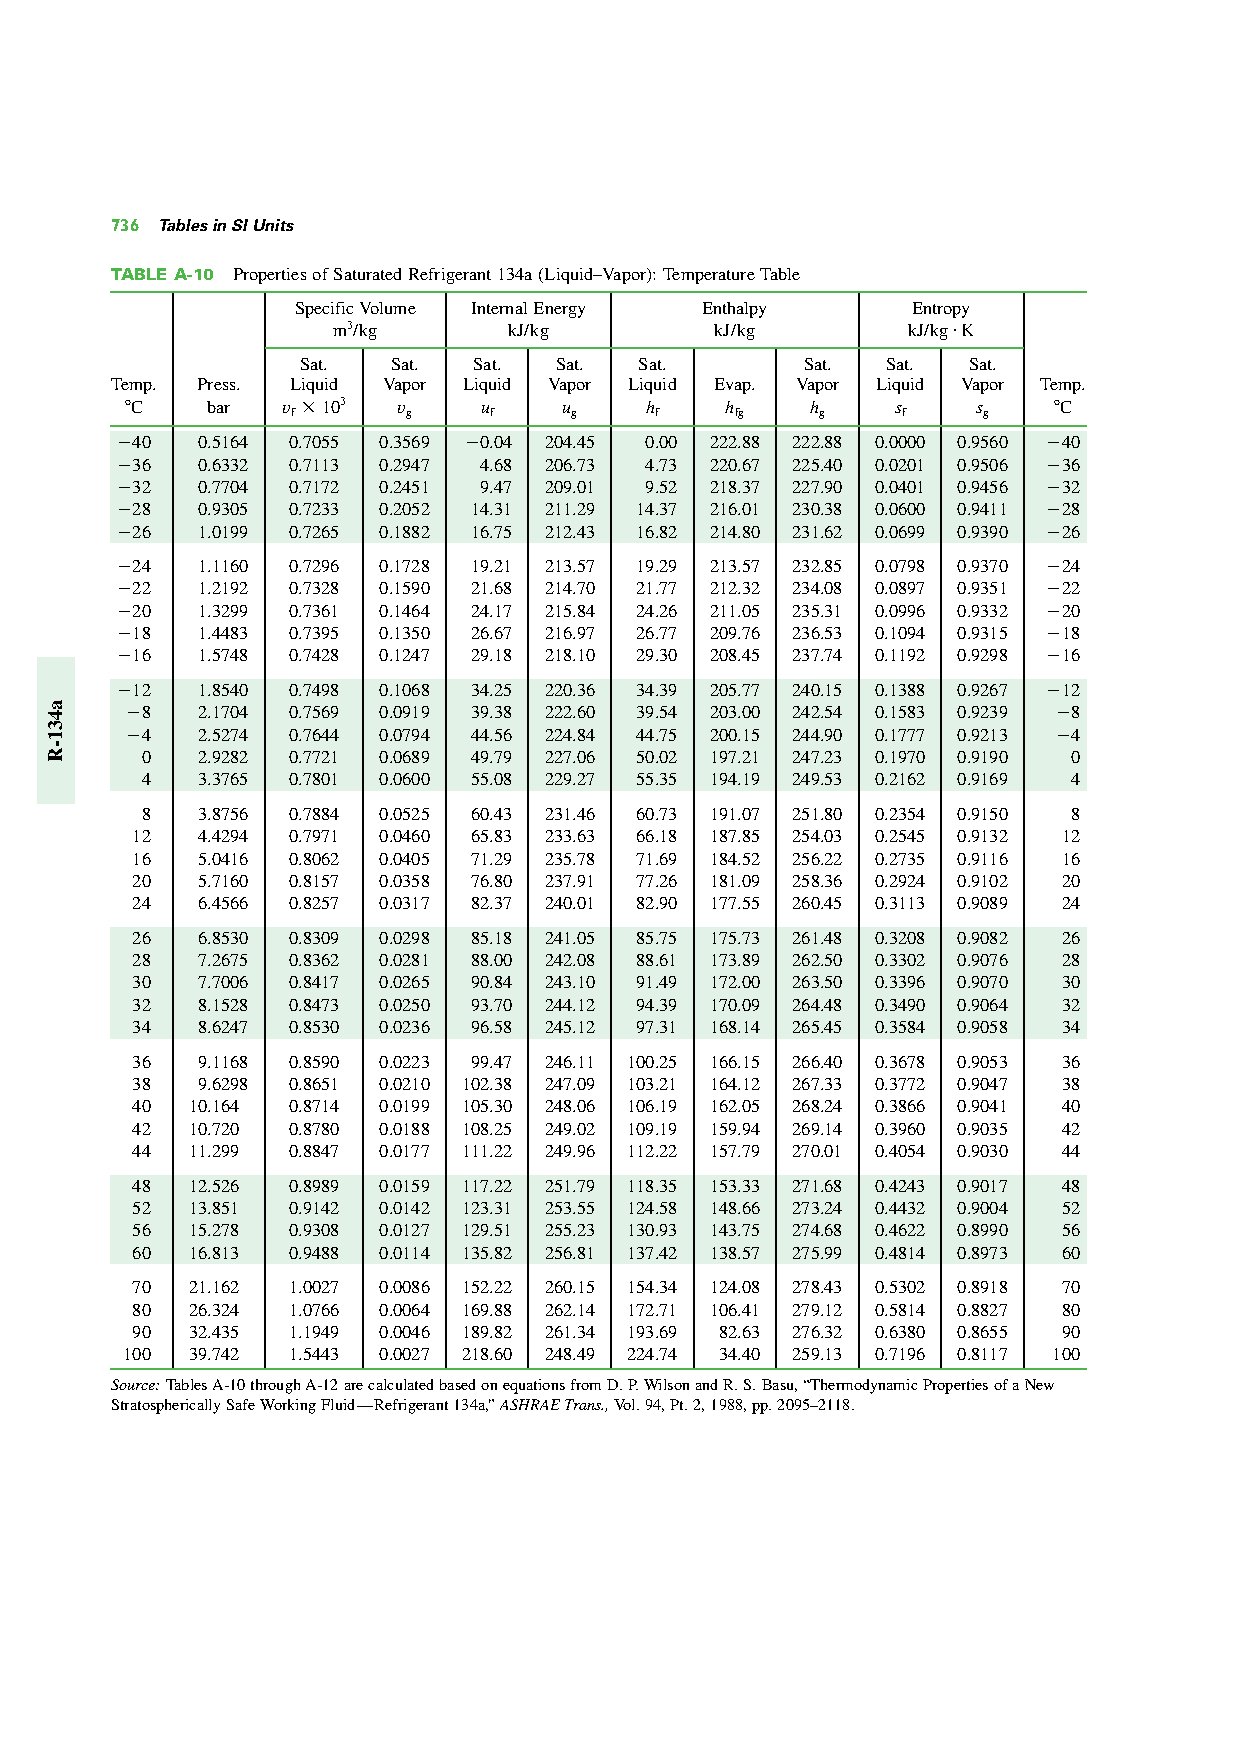
\includepdf[pages=-,fitpaper]{./Pics/Tables_R134}
%}
%\end{landscape}
%\end{comment}

\end{document}
